\chapter{Electron-Ion Collider}\label{cha:EIC} % chktex 24

The Electron-Ion Collider (EIC) is a planned accelerator facility to be built at Brookhaven National Laboratory [cite BNL] in the place of today's Relativistic Heavy Ion Collider (known as RHIC). Contrary to RHIC, which was built as an ion-ion collider, EIC will open new possibilities of probing the structure of nucleons by colliding the more complicated ions  with the comparably "simple-structured" electrons. Its versatile design will allow for the usage of a wide range of these ions: from protons (hydrogen ions) up to ions of uranium [cite Silvia DIS].

The key scientific questions to be addressed by EIC will be integrated into the final design of the whole accelerator complex, as well as of every experiment and its detectors within. One of these is investigating fundamental properties of nucleons, such as their mass and spin, and discovering how they emerge from the interactions of the partons (gluons and quarks) they are made of. Speaking of the partons, another puzzle for EIC is to solve how they are distributed inside nucleons, both in momentum and in position. It is also of high interest to discover how they interact with a nuclear medium, what makes the confined hadronic states emerge from these partons, and if the density of gluons keeps growing with increasing energies or if it reaches a point of saturation. [cite YR]

\section{From RHIC to EIC}
For more than twenty years RHIC has been a cornerstone of nuclear and particle physics. Commissioned in 2000, it was the first collider able to collide ions heavier than protons, creating the hot, dense conditions akin to those of the early Universe. [cite RHIC-facts] It was built as the result of a compromise between particle physicists interested in the mechanism of multiparticle production in high-energy hadron collisions and nuclear physicists interested in investigating the nuclear equation of state with the highly compressed nuclear matter. RHIC also pioneered the use of spin-polarized proton beams. [cite RHIC-program]

The legacy of innovation continues with the EIC, which will also incorporate a polarized electron beam into its design. The EIC will reuse much of the existing RHIC infrastructure, some of which are: the tunnel, cryogenic systems, and some of the magnets. The main changes will involve adding a new electron accelerator and modifying the existing ion accelerator to accommodate electron-ion collisions. This approach not only reduces costs but also leverages the proven capabilities of RHIC while significantly expanding its scientific reach.



EIC Hadron Storage Ring (HSR) to be composed of
existing arcs of the Yellow RHIC ring (remove
unused magnets)

\begin{figure}[H]
    \centering
    \begin{subfigure}{0.4\linewidth}
        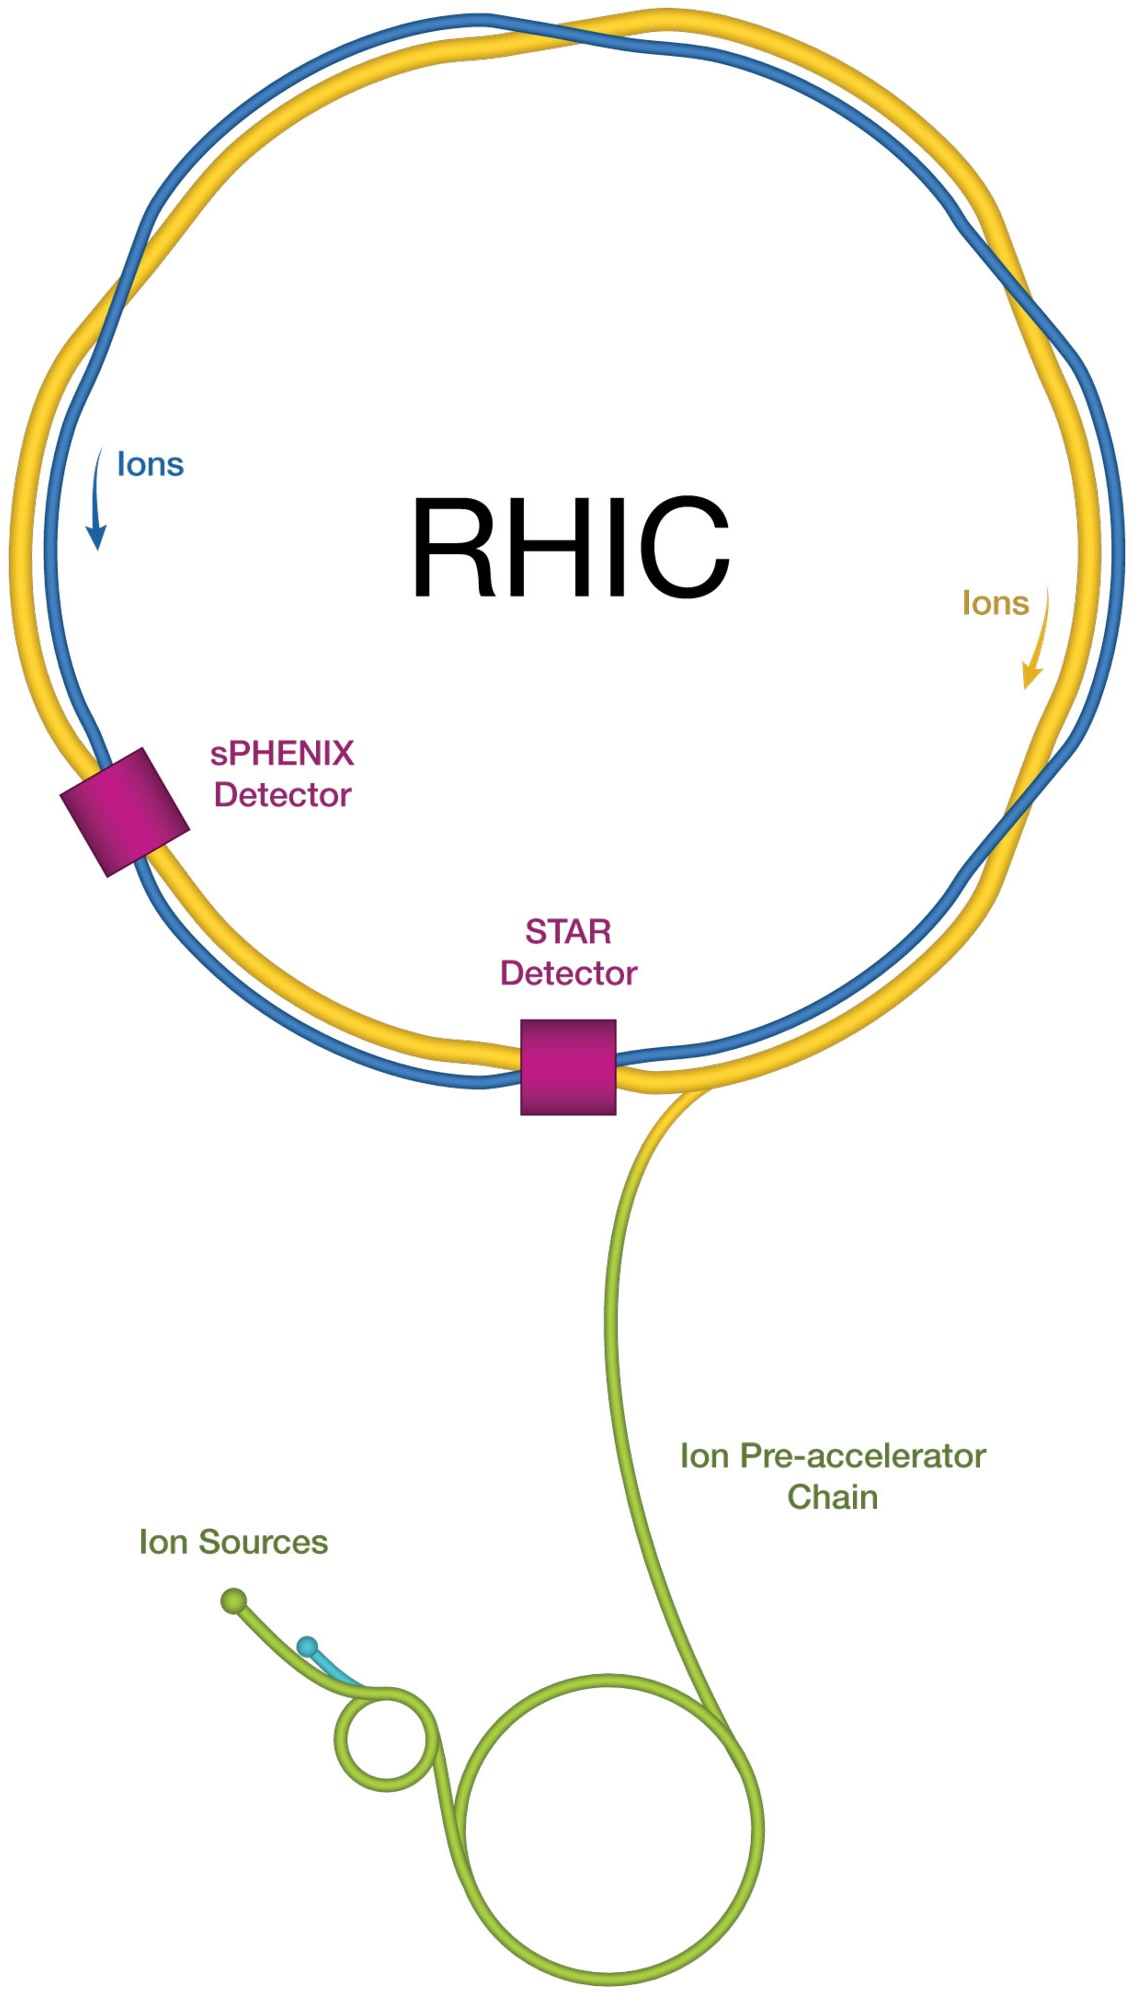
\includegraphics[height=10.4cm]{img/rhic.jpg}
        \caption{} % [cite RHIC image]
        \label{fig:eic:comparison::rhic}
    \end{subfigure}
    %\hspace{0.02\linewidth}
    \raisebox{20\height}{\Huge$\rightarrow$}
    %\hspace{0.02\linewidth}
    \begin{subfigure}{0.52\linewidth}
        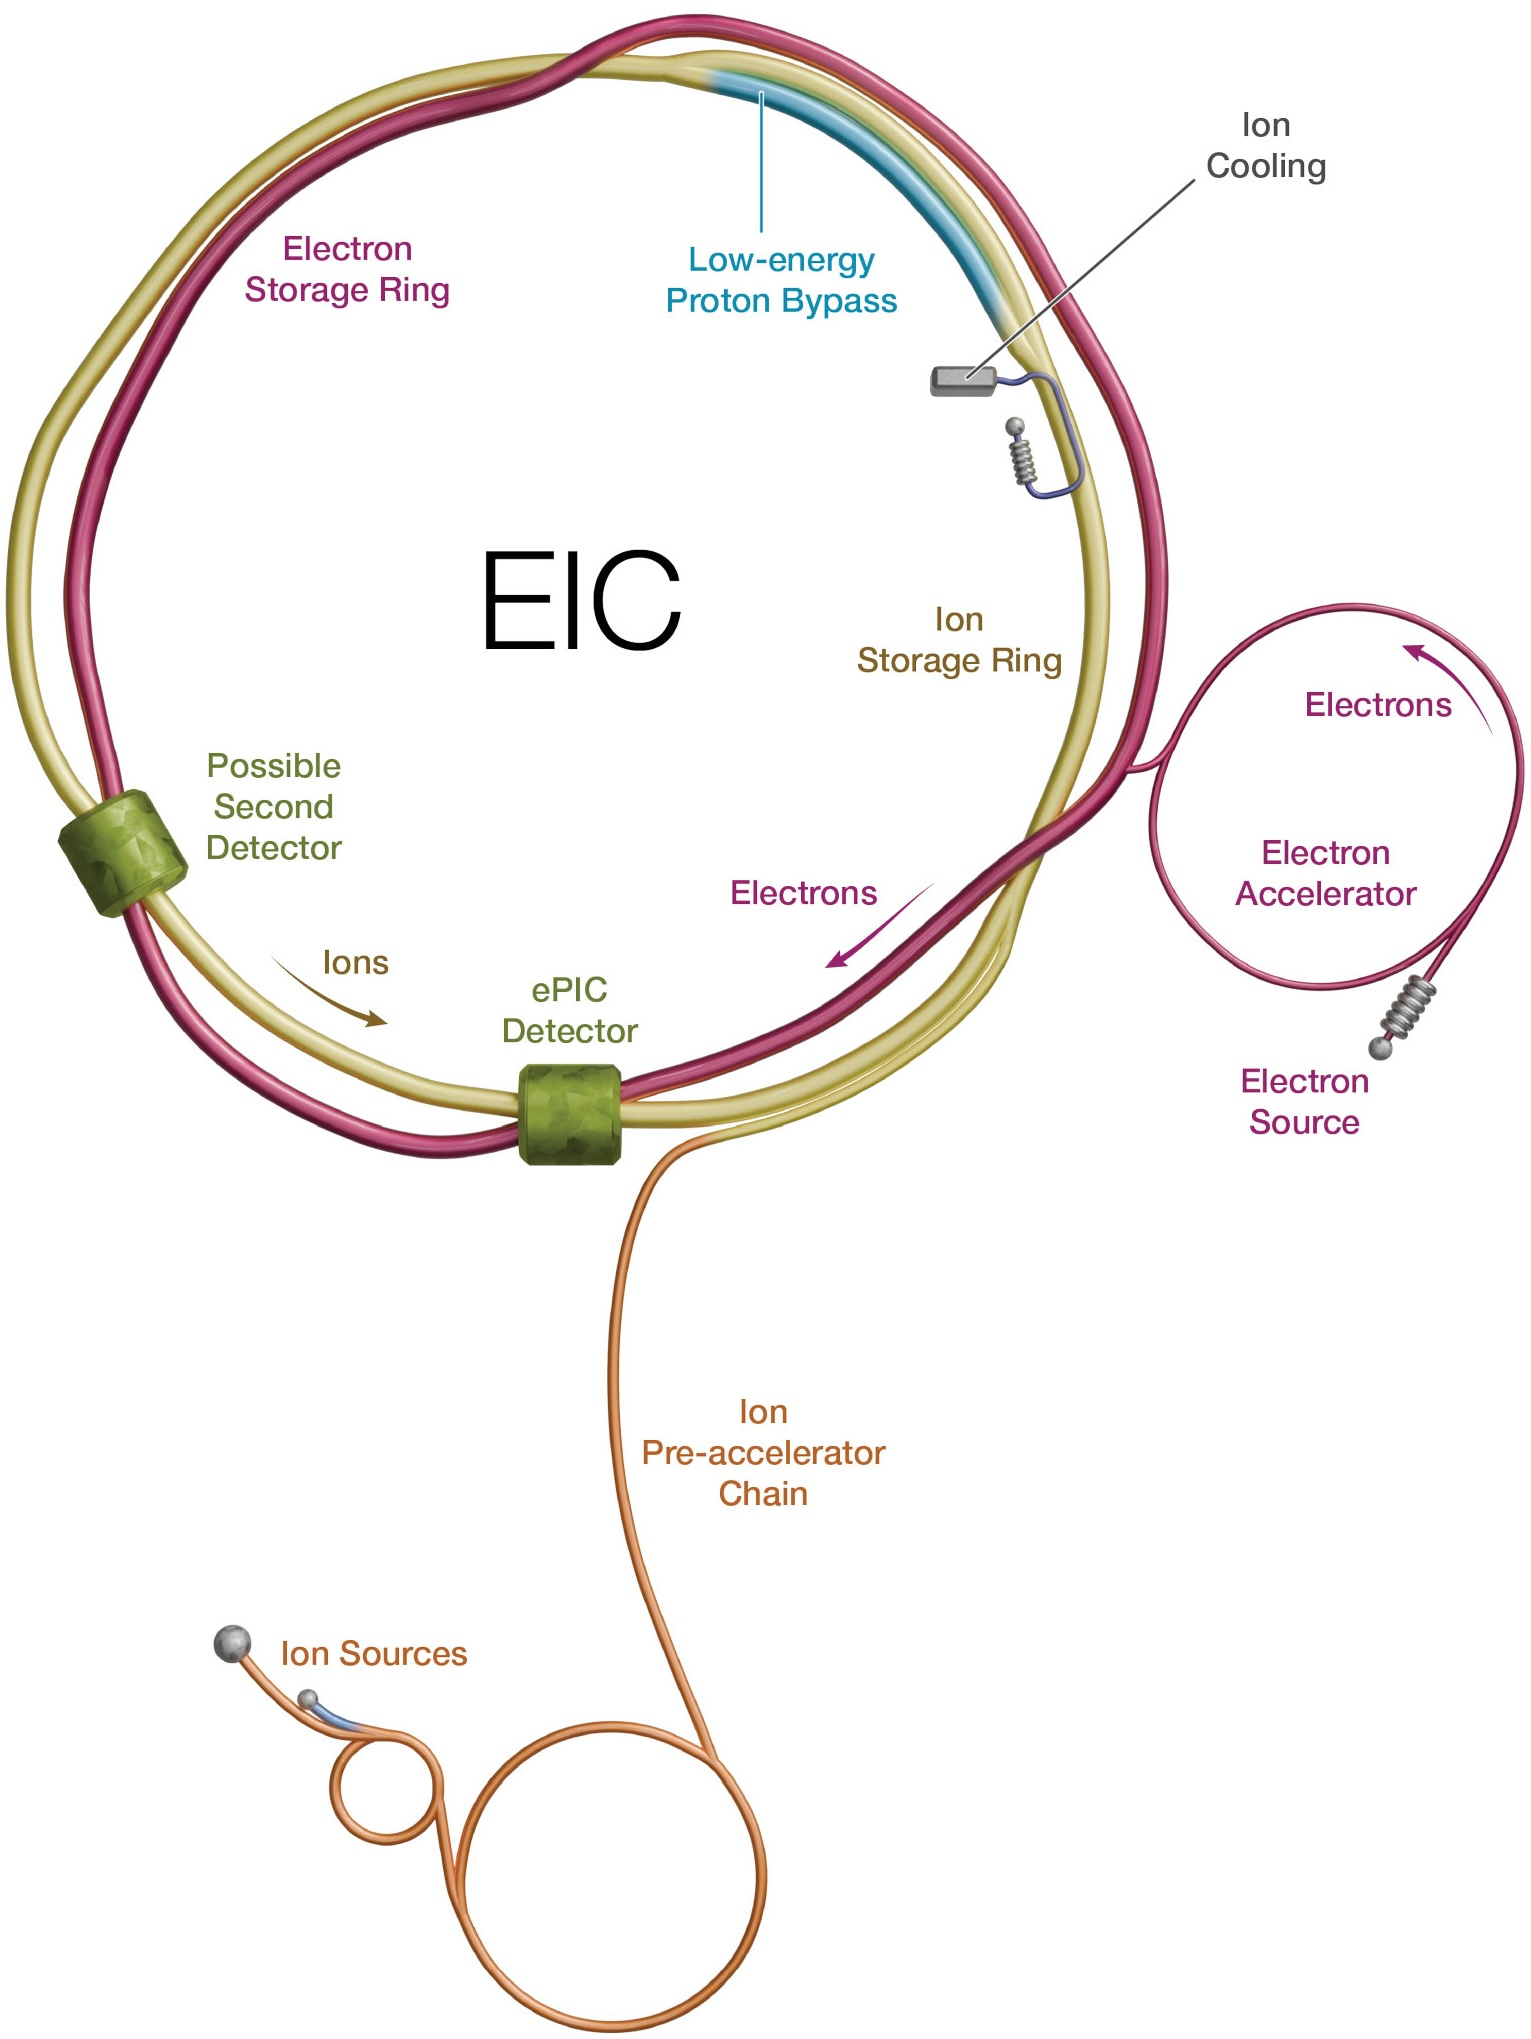
\includegraphics[height=10.4cm]{img/eic.jpg}
        \caption{} % [cite EIC image]
        \label{fig:eic:comparison::eic}
    \end{subfigure}
    \caption{(a) Layout of the existing RHIC facility. (b) Conceptual design of EIC.}
    \label{fig:eic:comparison}
\end{figure}

\begin{figure}[H]
    \centering
    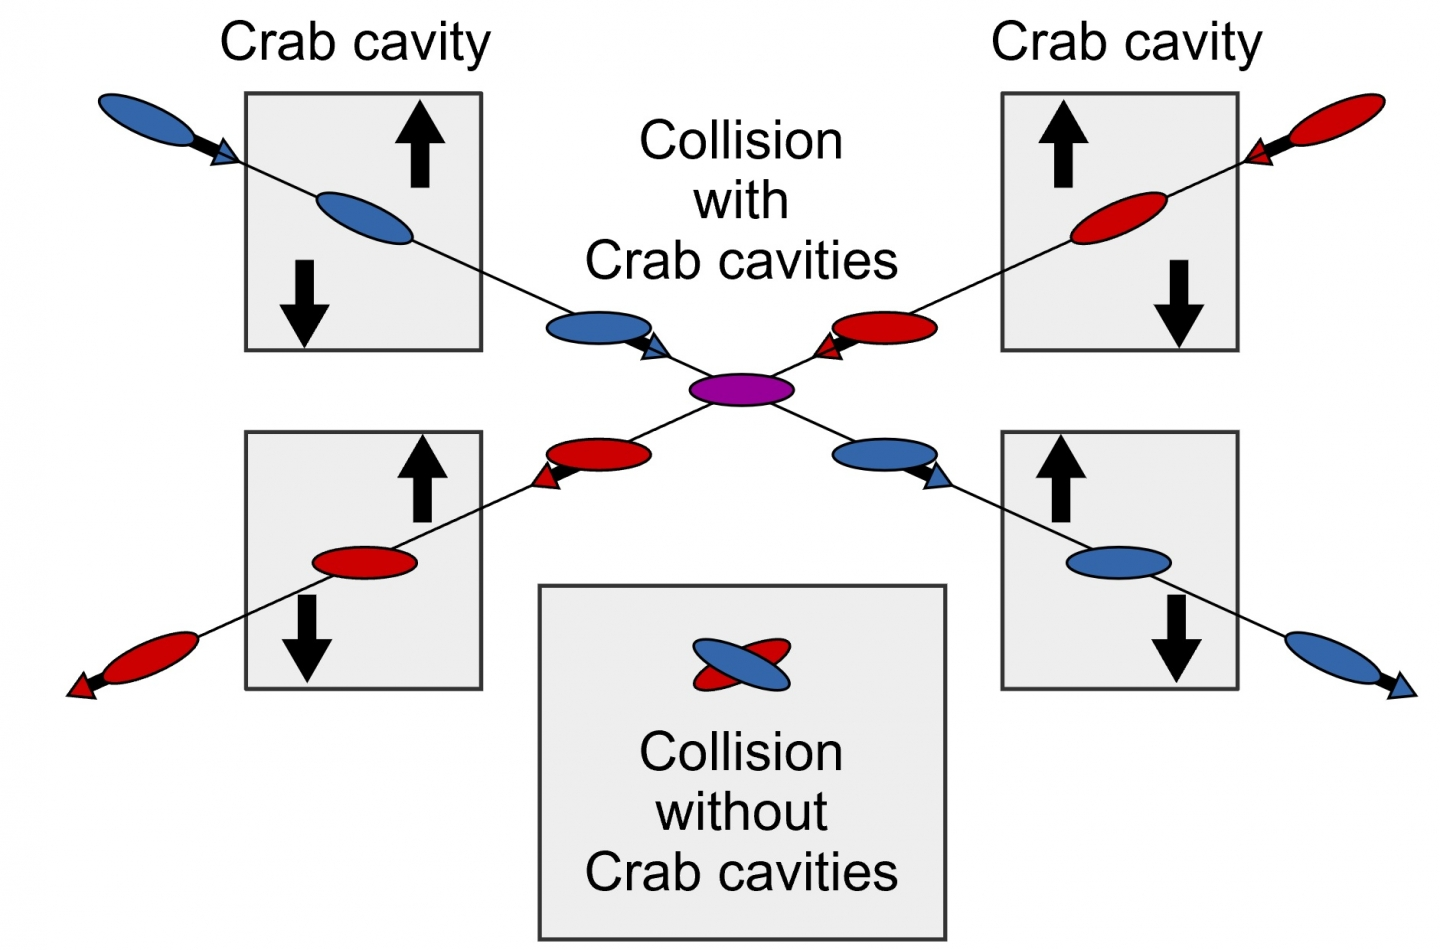
\includegraphics[width=.8\linewidth]{img/crab_cavities.jpg}
    %\caption{Crab cavities used to rotate the particle bunches before the collision to maximize the overlap of the colliding bunches. [cite EIC crab cavities]}
    \caption{Crab cavities. [cite crab-cavities]}
    \label{fig:eic:crab_cavities}
\end{figure}


\section{facts}


\section{Current Design Plan}

% \textit{the changes from usual illustrations (copied)}:\\
% In 2024, the project made several key EIC design decisions. They will lead to
% formal Project Scope changes after the Technical Change Control Board (TCCB)
% and the CCB processes.
% \begin{enumerate}[topsep=1mm, itemsep=0mm]
%     \item Reuse the entire Yellow RHIC ring, delay the 41-GeV bypass (a Blue RHIC arc).
%     \item Implement a new room-temperature Hadron Storage Ring (HSR) injection line.
%     \item Drop Strong Hadron Cooling (SHC), add Low-Energy Cooling (LEC).
%     \item Move the Rapid Cycling Synchrotron (RCS) out of the collider tunnel.
%     \item Delay the 28 nC/bunch and the 18 GeV capability implementation (ESR and RCS).
% \end{enumerate}
% These design decisions resolve uncertainties, challenges, and risks to EIC
% performance, safety, and future operation and maintenance. [Nagaitsev Frascati]


\section{AGS}

\section{RCS}

\section{Cooling}
Compared to HERA, the EIC design implements two new critical ideas:
\begin{enumerate}
    \item Flat proton bunches at collisions (to match the electron beam dimensions) - this helps with the
peak luminosity.
    \item Continuous proton beam cooling during collisions to maintain matched beam dimensions - this
helps with the average luminosity.
\end{enumerate}
\emph{The SHC-related risk was identified as HIGH.
To mitigate this risk, we are adding an injection electron cooler for hadrons (at 25 GeV/u) to create ‘flat’ bunches. This is a proven and tested technology. We propose to remove the SHC system from the project baseline.\\}
[Nagaitsev Frascati]

from Strong Hadron Cooler to Low Energy Electron Cooler (Ring Electron Cooler - something else?)

The Ring Electron Cooler must be located in the IR2 of the Hadron Storage Ring (HSR)





% maybe will fit better in another chapter

% \section{Advantages? \textit{Prínosy}}

% \section{Second detector?}
% is anyone seriously working on it, or is it too soon to care?

% \begin{figure}[H]
%     \centering
%     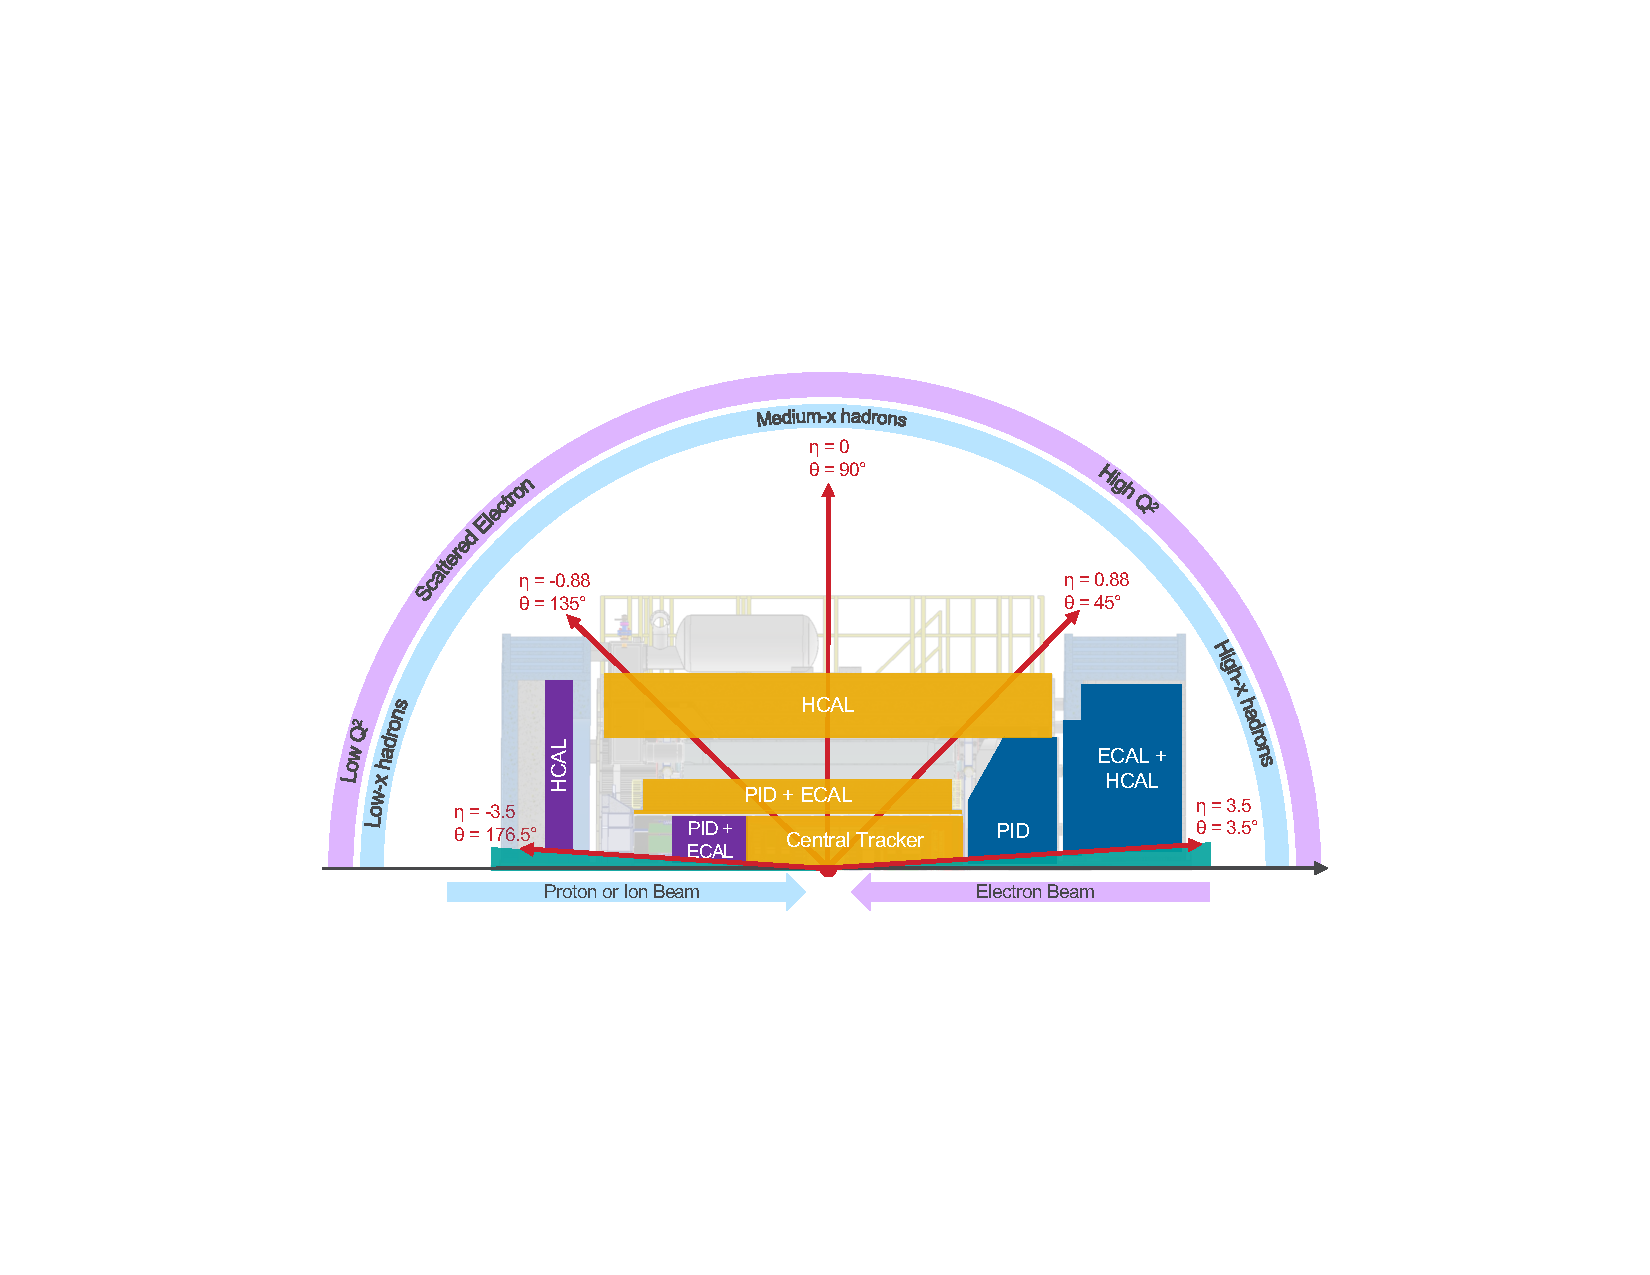
\includegraphics[width=.8\linewidth]{img/range.pdf}
%     \caption{always this image \url{https://doi.org/10.5281/zenodo.14939545}}
%     \label{fig:eic:range}
% \end{figure}